\documentclass[12pt]{article}

\usepackage[spanish]{babel}
\usepackage[none]{hyphenat}
\usepackage[left=1.5cm, right=1.5cm, top = 2cm, bottom=2.5cm]{geometry}
\usepackage{parskip}
\usepackage[export]{adjustbox}
\usepackage{enumitem}[shortlabels]
\usepackage{listings} 
\usepackage{color}
\usepackage{fancyhdr}
\usepackage{graphicx}
\usepackage{caption} 
% \usepackage{subcaption}
\usepackage{wrapfig}
% \usepackage{longtable}
% \usepackage{multirow, makecell}
% \usepackage{amsmath} 
\usepackage[hidelinks]{hyperref}
\usepackage{csquotes}

\newcommand{\linejump}{\hfill \break}
\renewcommand{\thefootnote}{\fnsymbol{footnote}}
% \newcommand{\unit}[1]{\ensuremath{\, \mathrm{#1}}}

\definecolor{dkgreen}{rgb}{0,0.6,0}
\definecolor{gray}{rgb}{0.5,0.5,0.5}
\definecolor{mauve}{rgb}{0.58,0,0.82}
\lstset{
  language=Java,
  aboveskip=3mm,
  belowskip=3mm,
  showstringspaces=false,
  columns=flexible,
  basicstyle={\scriptsize\ttfamily},
  numbers=none,
  numberstyle=\tiny\color{gray},
  keywordstyle=\color{blue},
  commentstyle=\color{dkgreen},
  stringstyle=\color{mauve},
  breaklines=true,
  breakatwhitespace=true,
  tabsize=2
}

\sloppy
\setlength{\parindent}{0cm}
\setlength{\columnsep}{0.5cm}
\decimalpoint
\graphicspath{{img/}}

\hypersetup{colorlinks=true, urlcolor=blue, citecolor=blue}
\urlstyle{same}

\pagestyle{fancyplain}
\fancyhf{}
\fancyhead[L]{\scriptsize 
  Universidad Nacional Autónoma de México \\
  Programación Orientada a Objetos \\
  M.C. Leonardo Ledesma Dominguez
}
\fancyhead[R]{\thepage}


\begin{document}
  \begin{center}
    Acosta Porcayo Alan Omar \\
    \linejump
    \LARGE \textbf{Tarea 6. UML Dinámico}
  \end{center}
  
  \linejump
  \begin{enumerate}
    \item Lea el capítulo II del libro Manual de UML de Paul Kimmel, y realice un resumen de una a dos cuartillas.
    
    \textbf{\large{El principio con casos de uso}} \\

    \textbf{Cómo hacer el caso para las casos de uso} \\
    La finalidad de un caso de uso es describir la manera en que se usará un sistema: describir sus finalidades esenciales. La finalidad de los diagramas de casos de uso es captar en forma visual las finalidades esenciales.

    Los diagramas de casos constan de figuras de línea, líneas y óvalos. La figura de palillos se llama actor y representa a alguien o algo que actúa sobre el sistema. Las líneas son punteadas o continuas, con varias flechas o sin ellas, que indican la relación entre el actor y los óvalos. Estos últimos son los casos de uso y, en el diagrama de casos de uso, los óvalos tienen algún texto que proporciona una descripción básica.

    En esencia, los casos de uso son listas de cosas por hacer. Una vez que ha captado los casos de uso, ha articulado lo que el sistema hará, y puede usar la lista para dar prioridades a las tareas.

    Una figura de palillos, una línea y un óvalo son suficientemente simplistas, cuando se combinan con algún texto, para que todos los participantes puedan entender el significado. El resultado es que los usuarios y clientes pueden observar los dibujos y leer el texto llano, y determinar si los tecnólogos han, o no, registrado con exactitud y comprendido las características deseables.

    Debido a que los casos de uso son visuales y sencillos, los usuarios y clientes pueden suministrar retroalimentación, y las personas que constituyen el puente entre los clientes y los programadores, como los administradores, pueden determinar si las características que en realidad se estructuraron reflejan con exactitud los deseos de los usuarios.

    \textbf{Uso de los símbolos de los casos de uso} \\
    Los actores se descubren como resultado del análisis. Conforme vaya identificando los macrousos del sistema, identificará quiénes son los participantes para esos casos de uso.

    El símbolo del caso de uso se utiliza para representar capacidades. Al caso de uso se le da un nombre y una descripción mediante un texto. Este último debe describir cómo inicia y finaliza el caso de uso, e incluye una descripción de la capacidad descrita por el nombre de la misma, así como escenarios de apoyo y requisitos no funcionales.

    Dado que los diagramas de casos de uso tienen múltiples actores y en virtud de que los casos de uso pueden estar asociados con los actores y con otros casos de uso, se utilizan los conectores para indicar la manera en que ambos están asociados. Los estilos de conectores pueden cambiar para transmitir más información acerca de la relación entre los actores y los casos de uso.

    Existen tres estilos básicos de líneas para los conectores. Un conector de línea simple se llama asociación y se usa para mostrar cuáles actores están relacionados con cuáles casos de uso. Un segundo estilo de conector es una línea punteada con una flecha direccional que se conoce como dependencia. Un tercer estilo de conector es una línea dirigida con un triángulo hueco, al cual se le conoce como generalización.

    Una notación más común en los conectores es el estereotipo. Los estereotipos agregan detalles a la relación entre los elementos en un diagrama de caso de uso. Se puede usar un estereotipo para ampliar el significado de este conector.

    Una relación de dependencia entre dos casos de uso significa que, de alguna manera, el caso dependiente necesita al caso del que depende. Dos estereotipos de uso común y predefinidos que refinan las dependencias en los casos de uso son el incluir y el extender.

    Una relación de dependencia entre dos casos de uso significa que, de alguna manera, el caso dependiente necesita al caso del que depende. Dos estereotipos de uso común y predefinidos que refinan las dependencias en los casos de uso son el incluir y el extender. El estereotipo extender se usa para agregar más detalle a una dependencia, lo cual significa que estamos agregando más capacidades

    Todos los diagramas, incluyendo los casos de uso, permiten que se les agreguen anotaciones en forma de texto. Las notas se representan como un trozo de papel con una punta doblada y una línea que une el cuadro de texto al elemento que se le está haciendo la anotación.

    \textbf{Creación de los diagramas de casos de uso} \\
    La suficiencia es un problema difícil. Si proporciona demasiados casos de uso, su modelado puede continuar durante meses o incluso años. Una línea de base razonable es que las aplicaciones de mediana complejidad podrían tener entre 20 y 50 buenos casos de uso.

    El objetivo de crear diagramas de casos de uso es documentar los importantes del sistema, para proporcionar a los usuarios una manera de baja tecnología para evaluar en forma visual sus comprensiones mutuas y, a continuación, seguir adelante.

    \textbf{Diseño controlado con casos de uso} \\
    Demasiados proyectos pasan por alto por completo los casos de uso e ignoran el establecimiento de prioridades, pero los casos de uso existen para ayudarle a administrar el alcance y para establecer prioridades. 
    
    El término diseño controlado por casos de uso significa que expresamos lo que estamos estructurando en nuestros casos de uso con el fin de limitar el alcance y evitar el desperdicio de tiempo, y establecemos prioridades en lo que estructuramos empezando con las características más críticas y de prioridad más alta.

    Después de que haya definido sus casos de uso, querrá establecer prioridades y además diseñar e implementar una solución para apoyar aquellos casos de uso con la prioridad más alta o que representan el riesgo más significativo. Esto se logra preguntando al cliente qué es lo más riesgoso, lo más importante o lo más valioso y a continuación enfocar sus energías en esos casos de uso.

    Lo importante aquí es la identificación de los casos de uso para establecer prioridades en la lista de tareas e ilustrar un camino crítico para el criterio de éxito mínimo.

    \newpage
    \item Investigue en que consiste la Persistencia de Objetos en Java. Mencione al menos dos aplicaciones de la Persistencia de Objetos.
    
    \textbf{Concepto:} \\
    La persistencia es la propiedad de un objeto a través del cual su existencia trasciende en el tiempo y/o espacio. Esto significa que un objeto persistente sigue existiendo después de que ha finalizado el programa que le dio origen y que además puede ser movido de la localidad de memoria en la que fue creado.

    El atributo de persistencia solamente debe estar presente en aquellos objetos que una aplicación requiera mantener entre corridas, de otra forma se estarían almacenando una cantidad probablemente enorme de objetos innecesarios. La persistencia se logra almacenando en un dispositivo de almacenamiento secundario (disco duro, memoria flash) la información necesaria de un objeto para poder restaurarlo posteriormente. Típicamente la persistencia ha sido dominio de la tecnología de base de datos.

    El lenguaje de programación Java permite serializar objetos en un flujo de bytes. Dicho flujo puede ser escrito a un archivo en disco y posteriormente leído y deserializado para reconstruir el objeto original. Con esto se logra lo que se llama "persistencia ligera" (\textit{lightwigth persistence} en inglés). 

    \textbf{Aplicaciones:}
    \begin{itemize}
      \item Aplicaciones de oficina: Las aplicaciones de oficina, como Microsoft Office, utilizan la persistencia de objetos para almacenar documentos, hojas de cálculo y presentaciones.
      \item Aplicaciones móviles: Las aplicaciones móviles utilizan la persistencia de objetos para almacenar datos de usuario, como contactos, calendario y preferencias.
      \item Juegos: Los juegos utilizan la persistencia de objetos para almacenar datos de usuario, como la configuración, el progreso y el estado del juego.
    \end{itemize}
  
    \newpage
    \item Realice el diagrama de actividades de un sistema de agenda de citas de un médico.
    
    \linejump
    \begin{figure}[ht]
      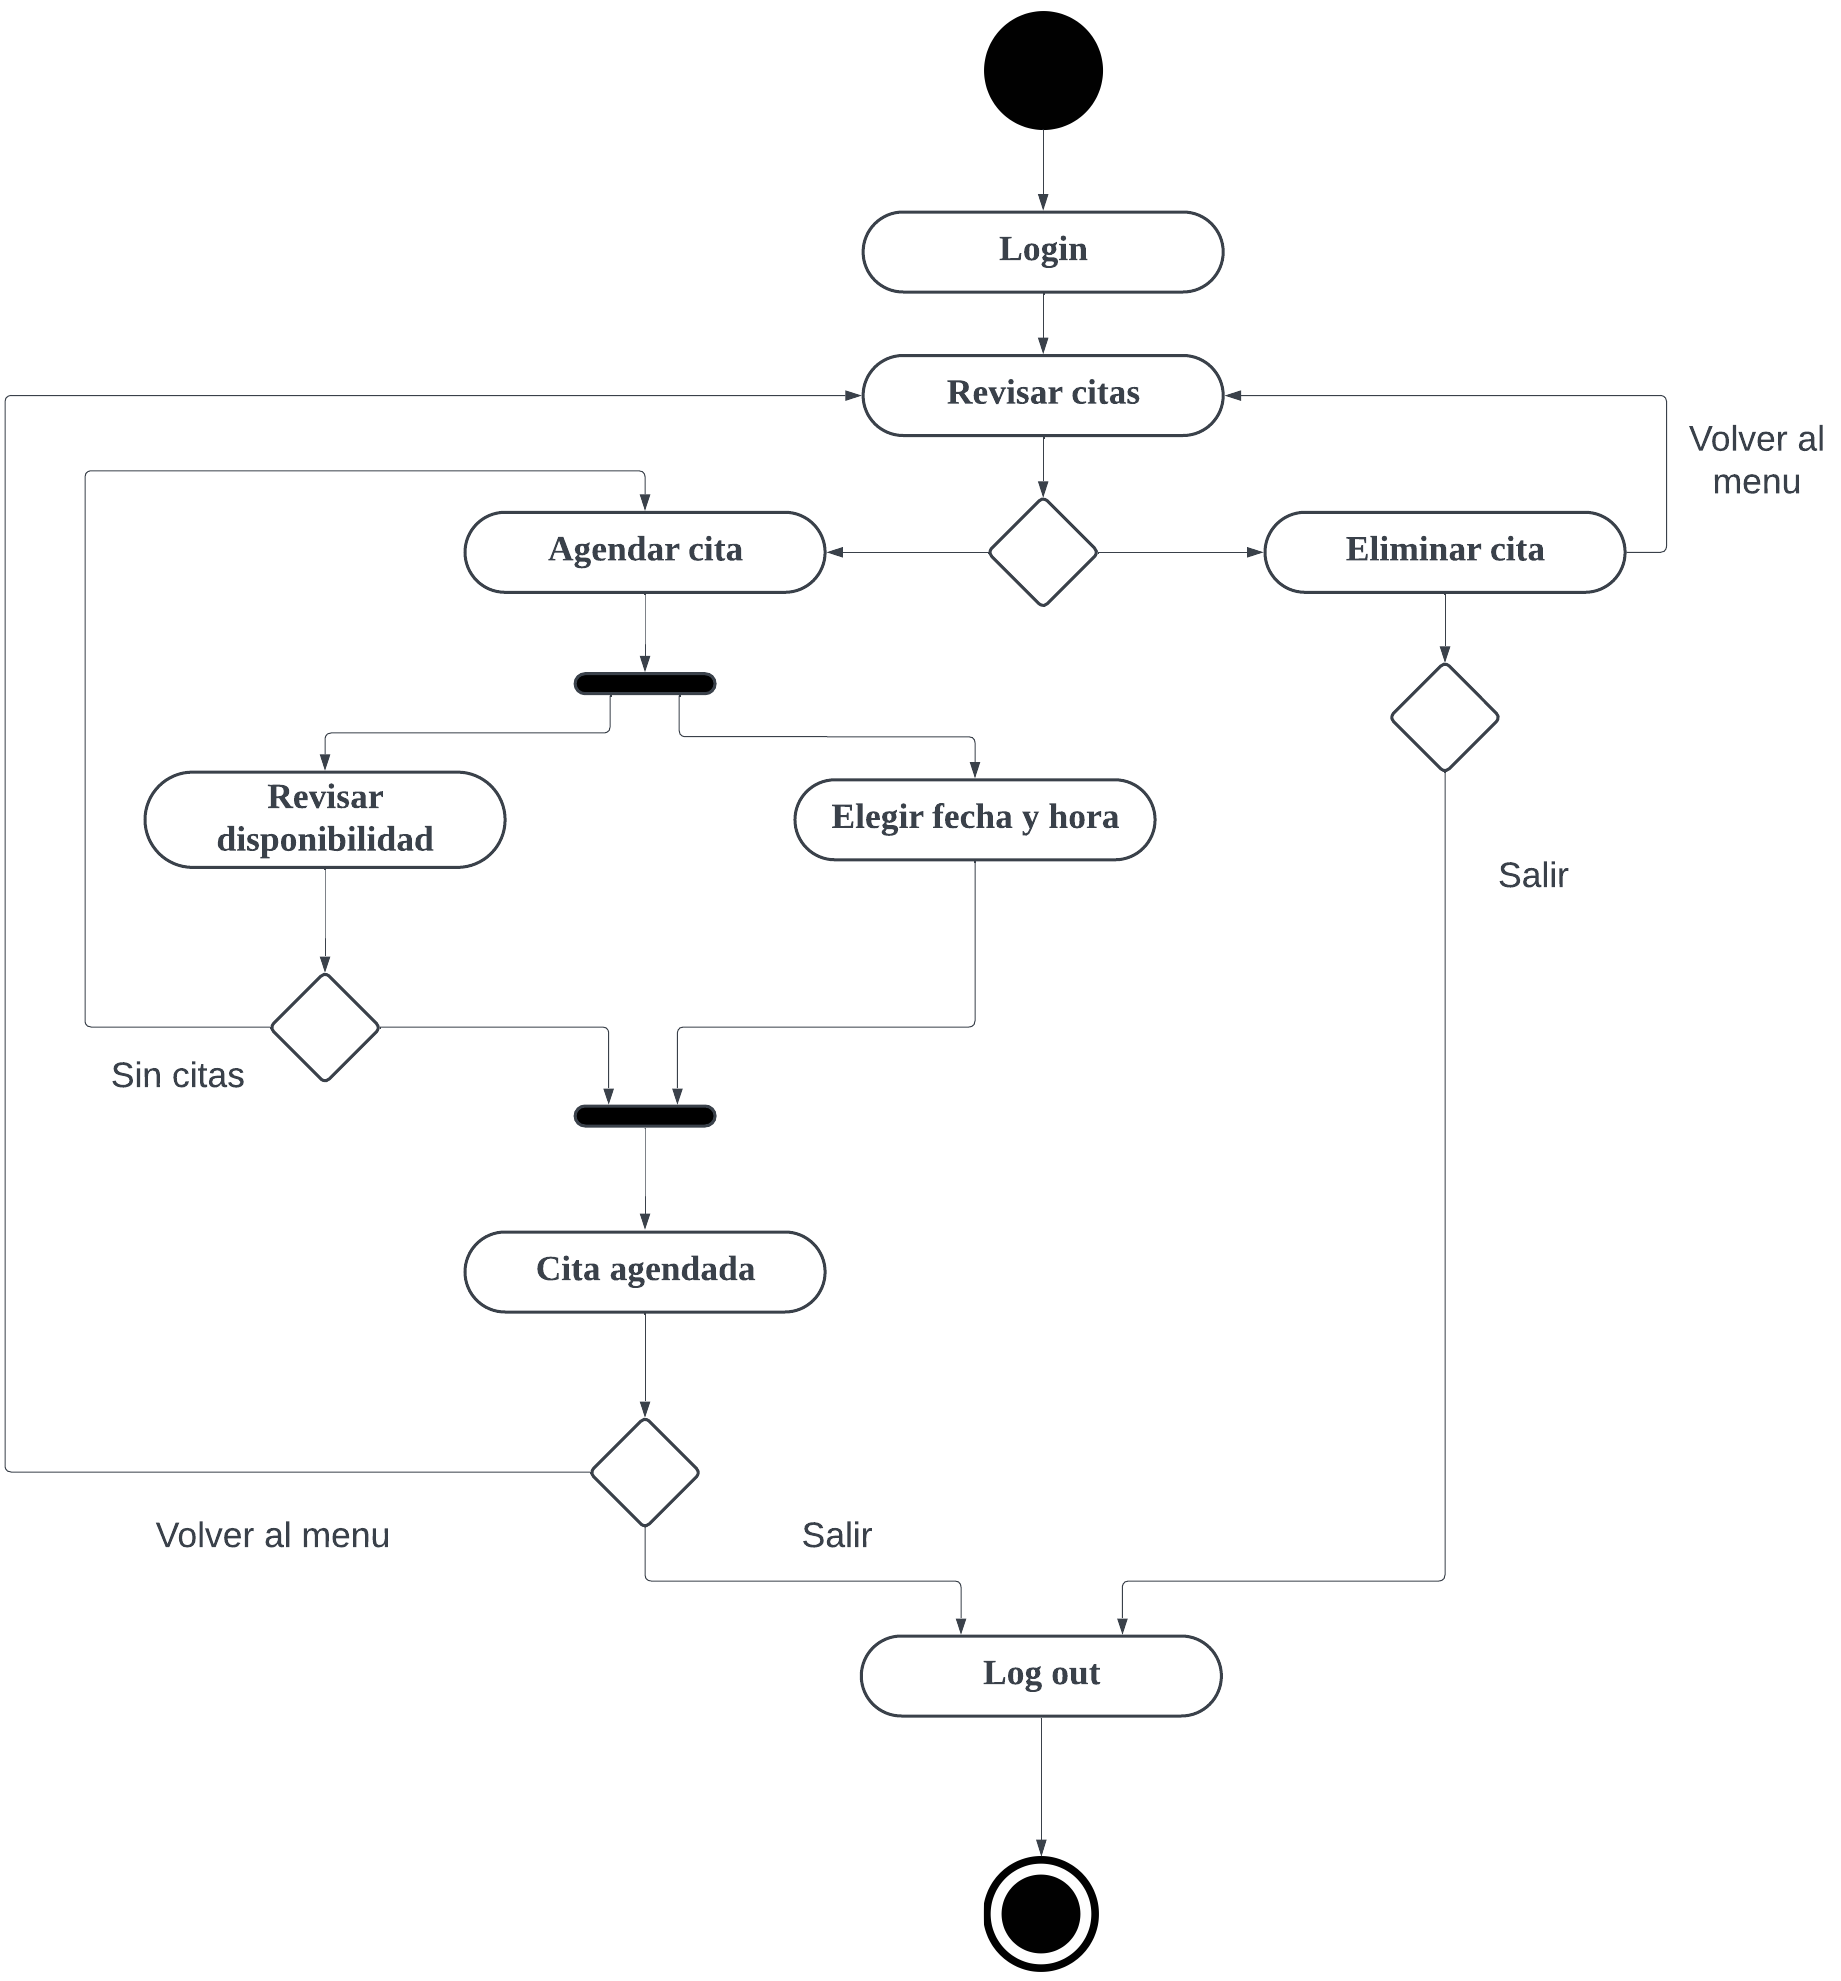
\includegraphics[width = 0.9\textwidth, center]{actividades.png}
    \end{figure}
    
    \newpage
    \item Realice el diagrama de estados del objeto Voto en el siguiente código:
    \begin{lstlisting}
public class Voto {
  private int INE = null;
  private boolean puedeVotar = null;
  
  Voto() {
    this.puedeVotar = existenciaINE();
  }
  
  private boolean existenciaINE() {
    return (PADRON.containsKey(INE)) ? true : false;
  }

  public boolean getPuedeVotar() {
    return puedeVotar;
  }
}

public class Elecciones {
  public static void main(String[] args) {
    Voto miVoto = new Voto();
    boolean regresar = false;

    do {
      if (miVoto.getPuedeVotar()) {
        emitirVoto();
      } else if(verificarCausa()) {
        emitirVoto();
      } else {
        regresar = invalidezVoto();
      }
    } while(regresar);
  }
}
    \end{lstlisting}
    \begin{figure}[ht]
      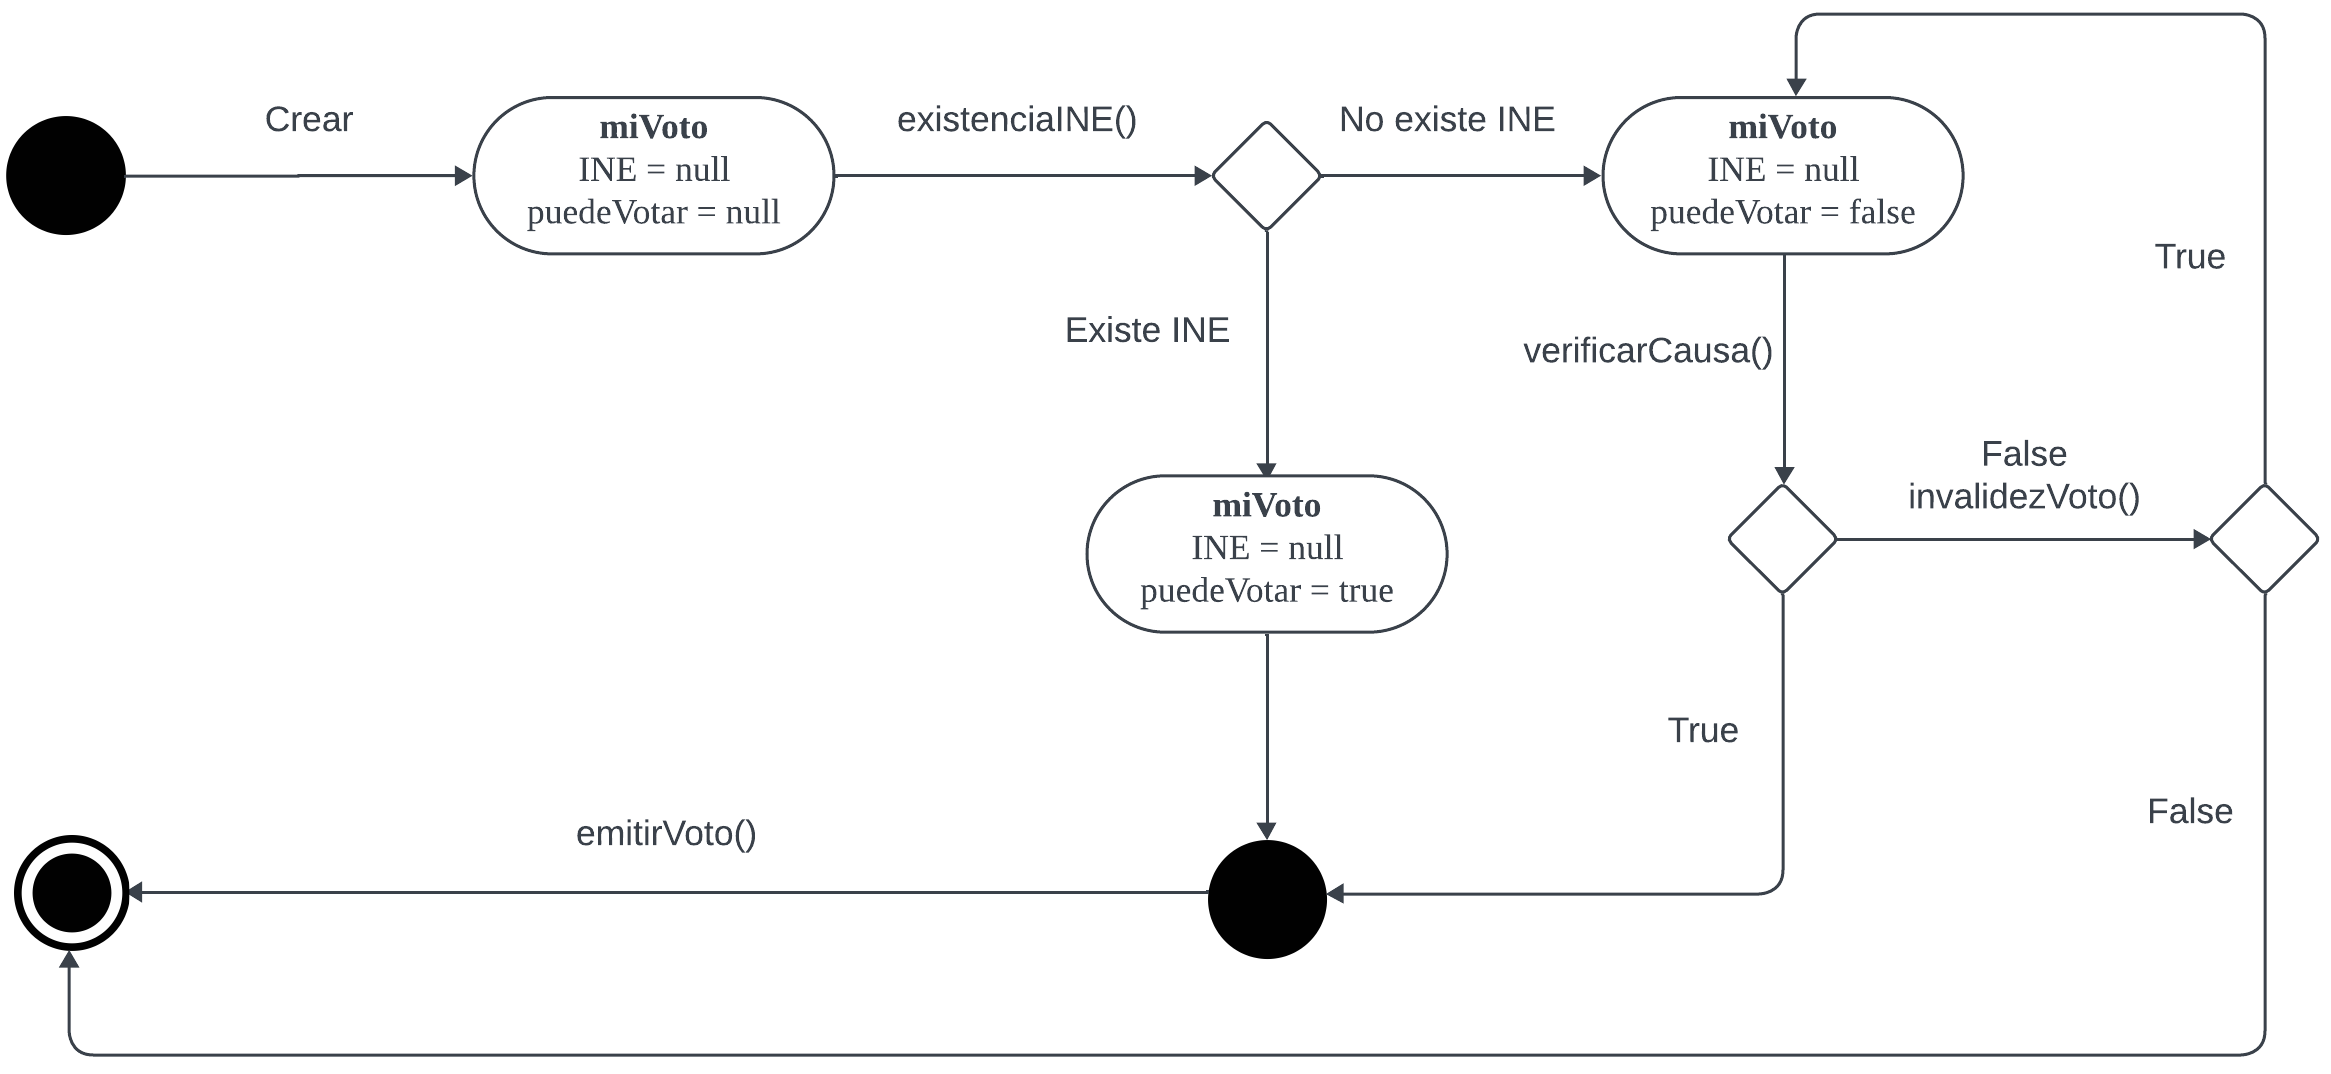
\includegraphics[width = \textwidth, center]{estado.png}
    \end{figure}
  \end{enumerate}

  \section*{Referencias}
  Ortiz, A. (n.d.). \textit{Persistencia en Java}. \url{https://arielortiz.info/apps/s201411/tc1018/notas_persistencia/} \\

  Paul, K. (2007). \textit{Manual de UML.} 
\end{document}